% inspired from http://tex.stackexchange.com/questions/47469/how-do-i-make-an-unbalanced-binary-tree and
% http://tex.stackexchange.com/questions/268128/how-to-nicely-place-two-heaps-next-to-each-other
\documentclass{article}
\usepackage[top=0.5in, bottom=1.25in, left=0.5in, right=0.5in]{geometry}

\usepackage{tikz}
\usetikzlibrary{trees}
\usetikzlibrary{shapes, positioning, arrows, calc}

\begin{document}

% Intro : représentation des sous problèmes

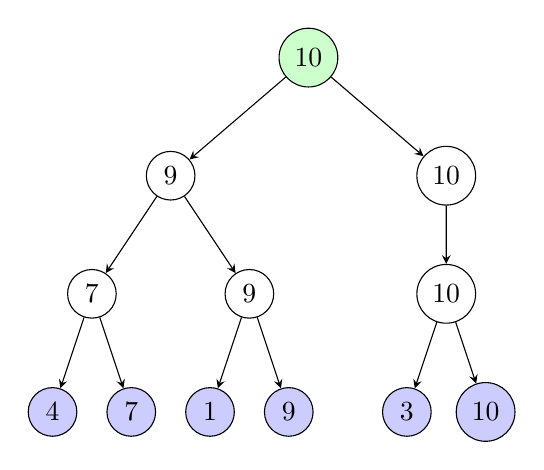
\begin{tikzpicture}[level distance = 1.5cm,
    level 1/.style={->, >=stealth, sibling distance=35mm},
    level 2/.style={->, >=stealth, sibling distance=20mm},
    level 3/.style={->, >=stealth, sibling distance=10mm}]
\tikzstyle{every node} = [circle, draw]
    \node[fill = green!20] {10}
        child {
	        node {9}
	        child { 
	        	node{7}
	        	child{node[fill=blue!20]{4}}
	        	child{node[fill=blue!20]{7}}
	        }
	        child {
	        	node {9}
	        	child{node[fill=blue!20]{1}}
	        	child{node[fill=blue!20]{9}}
	        }
    }
    child {
        node {10}
        child {
        	node{10}
        	child{node[fill=blue!20]{3}}
        	child{node[fill=blue!20]{10}}
        }
    };

\end{tikzpicture}

% Exemple arbre binaire

\vspace{2cm}

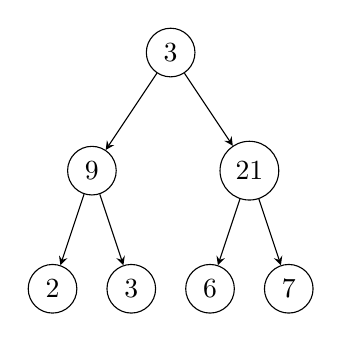
\begin{tikzpicture}[level distance = 1.5cm,
    level 1/.style={->, >=stealth, sibling distance=20mm},
    level 2/.style={->, >=stealth, sibling distance=10mm},
    level 3/.style={->, >=stealth, sibling distance=5mm}]
\tikzstyle{every node} = [circle, draw]
    \node{3}
        child {
	        node {9}
	        child{node{2}}
	        child{node{3}}
	    }
	    child {
	        node {21}
	        child{node{6}}
	        child{node{7}}
	    };

\end{tikzpicture}

% Exemple d'insertion de nœud dans un arbre binaire normal

\vspace{2cm}


\begin{tikzpicture}
\node[draw, circle] {A};
\end{tikzpicture}
\hspace{2cm}
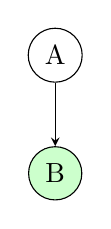
\begin{tikzpicture}[level distance = 1.5cm,
    level 1/.style={->, >=stealth, sibling distance=20mm},
    level 2/.style={->, >=stealth, sibling distance=10mm},
    level 3/.style={->, >=stealth, sibling distance=5mm}]
\tikzstyle{every node} = [circle, draw]
    \node{A}
        child{node[fill=green!20]{B}};
\end{tikzpicture}
\hspace{2cm}
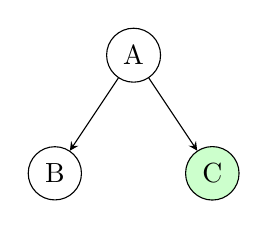
\begin{tikzpicture}[level distance = 1.5cm,
    level 1/.style={->, >=stealth, sibling distance=20mm},
    level 2/.style={->, >=stealth, sibling distance=10mm},
    level 3/.style={->, >=stealth, sibling distance=5mm}]
\tikzstyle{every node} = [circle, draw]
    \node{A}
        child{node{B}}
        child{node[fill=green!20]{C}};
\end{tikzpicture}
\hspace{2cm}
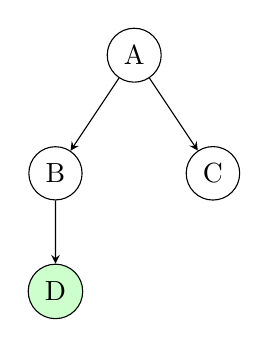
\begin{tikzpicture}[level distance = 1.5cm,
    level 1/.style={->, >=stealth, sibling distance=20mm},
    level 2/.style={->, >=stealth, sibling distance=10mm},
    level 3/.style={->, >=stealth, sibling distance=5mm}]
\tikzstyle{every node} = [circle, draw]
    \node{A}
        child{
        	node{B}
        	child{node[fill=green!20]{D}}
        }
        child{node{C}};
\end{tikzpicture}
\hspace{2cm}
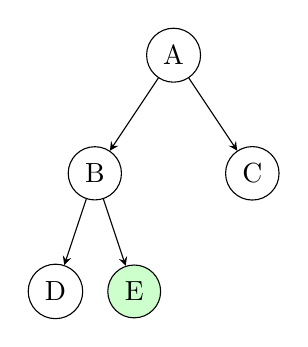
\begin{tikzpicture}[level distance = 1.5cm,
    level 1/.style={->, >=stealth, sibling distance=20mm},
    level 2/.style={->, >=stealth, sibling distance=10mm},
    level 3/.style={->, >=stealth, sibling distance=5mm}]
\tikzstyle{every node} = [circle, draw]
    \node{A}
        child{
        	node{B}
        	child{node{D}}
        	child{node[fill=green!20]{E}}
        }
        child{node{C}};
\end{tikzpicture}

% Exemple de suppression de nœuds (3 cas) dans un arbre binaire normal

\newpage

% Cas 1 : pas d'enfant

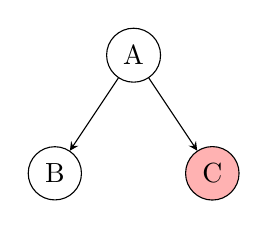
\begin{tikzpicture}[level distance = 1.5cm,
    level 1/.style={->, >=stealth, sibling distance=20mm},
    level 2/.style={->, >=stealth, sibling distance=10mm},
    level 3/.style={->, >=stealth, sibling distance=5mm}]
\tikzstyle{every node} = [circle, draw]
    \node{A}
        child{node{B}}
        child{node[fill=red!30]{C}};
\end{tikzpicture}
\hspace{2cm}
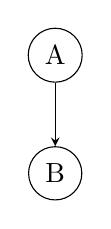
\begin{tikzpicture}[level distance = 1.5cm,
    level 1/.style={->, >=stealth, sibling distance=20mm},
    level 2/.style={->, >=stealth, sibling distance=10mm},
    level 3/.style={->, >=stealth, sibling distance=5mm}]
\tikzstyle{every node} = [circle, draw]
    \node{A}
        child{node{B}};
\end{tikzpicture}

% Cas 2 : un seul enfant

\vspace{2cm}

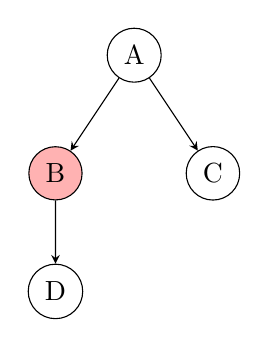
\begin{tikzpicture}[level distance = 1.5cm,
    level 1/.style={->, >=stealth, sibling distance=20mm},
    level 2/.style={->, >=stealth, sibling distance=10mm},
    level 3/.style={->, >=stealth, sibling distance=5mm}]
\tikzstyle{every node} = [circle, draw]
    \node{A}
        child{
        	node[fill=red!30]{B}
        	child{node{D}}
        }
        child{node{C}};
\end{tikzpicture}
\hspace{2cm}
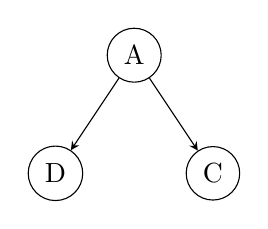
\begin{tikzpicture}[level distance = 1.5cm,
    level 1/.style={->, >=stealth, sibling distance=20mm},
    level 2/.style={->, >=stealth, sibling distance=10mm},
    level 3/.style={->, >=stealth, sibling distance=5mm}]
\tikzstyle{every node} = [circle, draw]
    \node{A}
        child{node{D}}
        child{node{C}};
\end{tikzpicture}

% Implémentation d'un arbre binaire dans un tableau

\vspace{2cm}

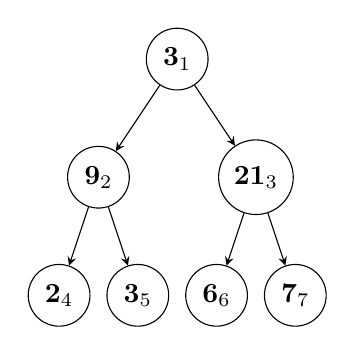
\begin{tikzpicture}[level distance = 1.5cm,
    level 1/.style={->, >=stealth, sibling distance=20mm},
    level 2/.style={->, >=stealth, sibling distance=10mm},
    level 3/.style={->, >=stealth, sibling distance=5mm}]
\tikzstyle{every node} = [circle, draw, font=\bfseries]
    \node{3$_1$}
        child {
	        node {9$_2$}
	        child{node{2$_4$}}
	        child{node{3$_5$}}
	    }
	    child {
	        node {21$_3$}
	        child{node{6$_6$}}
	        child{node{7$_7$}}
	    };

\end{tikzpicture}

\vspace{0.5cm}

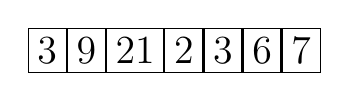
\begin{tikzpicture}
\node [font=\sffamily\Large\bfseries, draw, anchor=center] (first) {$3$};
\node [font=\sffamily\Large\bfseries, draw, anchor=center, right=0cm of first] (second) {$9$};
\node [font=\sffamily\Large\bfseries, draw, anchor=center, right=0cm of second] (third) {$21$};
\node [font=\sffamily\Large\bfseries, draw, anchor=center, right=0cm of third] (fourth) {$2$};
\node [font=\sffamily\Large\bfseries, draw, anchor=center, right=0cm of fourth] (fifth) {$3$};
\node [font=\sffamily\Large\bfseries, draw, anchor=center, right=0cm of fifth] (sixth) {$6$};
\node [font=\sffamily\Large\bfseries, draw, anchor=center, right=0cm of sixth] (seventh) {$7$};
\end{tikzpicture}

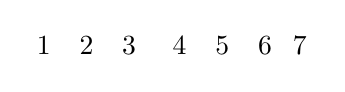
\begin{tikzpicture}
\node [font=\sffamily\Large\bfseries, anchor=center] (first) {$_1$};
\node [font=\sffamily\Large\bfseries, anchor=center, right=0.1cm of first] (second) {$_2$};
\node [font=\sffamily\Large\bfseries, anchor=center, right=0.1cm of second] (third) {$_3$};
\node [font=\sffamily\Large\bfseries, anchor=center, right=0.2cm of third] (fourth) {$_4$};
\node [font=\sffamily\Large\bfseries, anchor=center, right=0.1cm of fourth] (fifth) {$_5$};
\node [font=\sffamily\Large\bfseries, anchor=center, right=0.1cm of fifth] (sixth) {$_6$};
\node [font=\sffamily\Large\bfseries, anchor=center, right=0cm of sixth] (seventh) {$_7$};
\end{tikzpicture}

\end{document}